% Korttien lisääminen komennolla \k{x}{y}, missä x ja y ovat saman lausekkeen kaksi eri muotoa.

%switch sille, että minkä luokan kortit printataan.

%a-luokan kortit

%\begin{kortit}{A}
%
%
%\k{-2-(-5)}{3}
%
%\k{5-(-2)}{7}
%
%\k{5+(-x)}{5-x}
%
%\k{2+(+x)}{2+x}
%
%\end{kortit}

%b-luokan kortit jne.

%\begin{kortit}{B}
%	
%	
%\k{9\cdot x}{9x}
%
%\end{kortit}
%
%\begin{kortit}{C}
%	
%\k{\dfrac{15}{9}}{\dfrac{5}{3}}
%\k{\dfrac{30}{4}}{\dfrac{15}{2}}
%
%\k{\dfrac{x}{y}:\dfrac{x^2}{y^2}:\dfrac{x^3}{y^3}}{\dfrac{y^4}{x^4}}
%\k{\dfrac{-570}{9}}{\dfrac{190}{-3}}
%\k{\dfrac{1+x}{x}}{1+1/x}
%%\k{1/(1+1/x))}{x/(x+1)}
%
%\k{\dfrac{3x}{x}}{3}
%\k{\dfrac{3x^2}{x}}{3x}
%\k{\dfrac{3x^2}{6x}}{\dfrac{x}{2}}
%\k{\dfrac{3x}{x^2}}{\dfrac{3}{x}}
%\k{\dfrac{6x}{3x^2}}{\dfrac{2}{x}}
%\k{\dfrac{1}{3}x}{\dfrac{x}{3}}
%\k{\dfrac{6x^2}{x}}{6x}
%\k{\dfrac{2\cdot5\cdot 7}{10\cdot 7 \cdot 8}}{\dfrac{1}{8}}
%\k{\dfrac{1}{2}\cdot \dfrac{2}{3}\cdot \dfrac{3}{4}}{\dfrac{1}{4}}
%\k{\dfrac{x-1}{x^2-1}}{\dfrac{1}{x+1}}
%\k{\dfrac{x-1}{x^2-x}}{\dfrac{1}{x}}
%\k{\dfrac{x-1}{x^2-x^2}}{\text{ei määritelty}}
%\k{\dfrac{\dfrac{x^3}{10}}{\dfrac{x}{5}}}{\dfrac{x^2}{2}}
%\k{\dfrac{\dfrac{1+x}{x}}{\dfrac{x^2+x}{x^2}}}{1}
%\k{\dfrac{\dfrac{5}{6}}{\dfrac{6}{5}}}{\dfrac{25}{36}}
%\k{\dfrac{x^2(x-1)}{x+1}\cdot \dfrac{x+1}{x^2}}{x-1}
%\k{(x-a)(x-b)(x-c)\cdot \ldots \cdot (x-å)}{0}
%
%\k{\dfrac{1}{x}+\dfrac{1}{x^2}}{\dfrac{x+1}{x^2}}
%\k{\dfrac{1}{x}-\dfrac{1}{x^2}}{\dfrac{\dfrac{-2}{x^2}-\dfrac{-2}{x}}{2}}
%\k{\dfrac{1}{x}\cdot \dfrac{1}{x^2}}{\dfrac{1}{x^3}}
%\k{\dfrac{1}{x}:\dfrac{1}{x^2}}{x}
%
%
%\k{\dfrac{x^2-x+x(x+1)}{x^2}}{\dfrac{x-1+(x+1)}{x}}
%
%\k{\dfrac{x-1}{x}+\dfrac{x+1}{x}}{2}
%\k{\dfrac{x-1}{x}-\dfrac{x+1}{x}}{-\dfrac{2}{x}}
%\k{\dfrac{x-1}{x}\cdot \dfrac{x+1}{x}}{x-\dfrac{1}{x}}
%\k{\dfrac{x-1}{x}:\dfrac{x+1}{x}}{\dfrac{x-1}{x+1}}
%
%\k{\dfrac{x}{x-1}+\dfrac{x-1}{x}}{\dfrac{2x^2-2x+1}{x^2-x}}
%\k{\dfrac{x}{x-1}-\dfrac{x-1}{x}}{\dfrac{2x-1}{x^2-x}}
%\k{\dfrac{x}{x-1}\cdot \dfrac{x-1}{x}}{1}
%\k{\dfrac{x}{x-1}:\dfrac{x-1}{x}}{\dfrac{x^2}{x^2-2x+1}}
%
%\k{(a-1/a):(1-1/a)}{a+1}

%\end{kortit}

%\begin{kortit}{D}
%
%\k{\sin^2 x + \cos^2 x}{1}
%
%\k{\cos^2 x \sin x + \sin^3 x}{\sin x}
%\end{kortit}

%\kA{6x}{5x}
%
%\kA{t}{-2t}


%\kA{x+x-x+x}{2x}
%%

%\kA{x+x+x}{3\cdot x}

%vaihdantalakia ja liitäntälakia!

%\kA{3x+2x}{5x+x}
%

%
%\kA{-(1-x)}{-(y-2)}
%
%\kA{2-y}{x-1}


%\kA{3t-2t}{-3t+t}
%
%\kA{x(a-1)}{ax-x}
%
%\kA{a(x-1)}{ax-a}
%
%\kA{a(1-x)}{a-ax} 
%
%\kA{x(1-a)}{x-ax}


%\kA{\dfrac{x-1}{1-x}}{-1} %B:tä jo?

%\kA{3-3\cdot3}{-6}
%
%\kA{3\cdot3-3}{6}
%
%\kA{(3-3)\cdot3}{0}
%
%\kA{x-2(2x+4)}{-3x-8}
%
%\kA{2(2x-4)-x}{3x-8}
%
%\kA{2t-3t(x-t)\cdot 0}{2t}
%paljon murtolukuja eri muodoissa
%\kA{2t\cdot 0-3t(x-t)}{-3tx+3t}
%kertomerkki -yms. merkitsemiskäytännöt, selvä ero pystyyn kirjoitetutlle ja kursiiville
% yksikköpyörittelyä
%\kA{2(2x-4)-x}{3x-8}
%

%
%\kA{2(6-1)}{10}
%
%\kA{-2(x+1)}{-2x-2}
%
%\kA{-2(x-1)}{-2x+2}
%
%\kA{2(1-6)}{-10}
%
%\kA{(-1)(-2)}{2}
%
%\kA{(-1)(-2)(-1)}{-2}

%
%
%\kB{\dfrac{5}{10}}{\dfrac{6}{10}}
%
%\kB{\dfrac{2x}{x}}{\dfrac{-4x}{2x}}
%
%\setcounter{lauseke}{1}
%
%\kC{y(y^2-1)}{y^2(y-1)}
%
%\kC{y^3-y^2}{y^3-y}

%\k{1\frac{1}{2}}{1+\frac{1}{1}} %+murtoluvusta desimaaliiin jne.

%mikä aksiooma?
%\begin{kortit}{E}
%%\k{2+3}{3+2}
%%\k{x+y}{y+x}
%\k{x^2+3}{3+x^2}
%\k{(-1)+3}{3+(-1)}
%\k{(1+2)+3}{3+(1+2)}
%\k{(a+b)+c}{(b+a)+c}
%\k{(a+b)+c}{a+(b+c)}
%\k{(a+b)+c}{c+(a+b)}
%\k{-a+b}{b+(-a)}
%\k{\dfrac{1+x}{x}}{\dfrac{x+1}{x}}
%\k{-\pi+x^5}{x^5+(-\pi)}
%\k{2\sin(x)+\sqrt{y}}{\sqrt{y}+2\sin(x)}
%
%\k{b+(-b)}{b-b}
%
%\k{b+(-b)}{0}
%
%\k{x+(-y)}{x-y}
%
%\k{(y+(-7))+x}{y+(-7)+x}
%\k{(y+(-7))+x}{y+((-7)+x)}
%\k{(y+(-7))+x}{((-7)+y)+x}
%\k{(y+(-7))+x}{(y-7)+x}
%\k{(y+(-7))+x}{x+(y+(-7))}
%
%\end{kortit}

%\begin{kortit}{J} %vastaluku ja vähennyslaskun määritelmä
%\k{x+(-1)}{x-1}
%\k{-x+(-1)}{-x-1}
%\k{-x-(-1)}{1-x}
%\k{1-(-x)}{1+x}
%\k{-2-x}{-2+(-x)}
%\k{2-(+x)}{2-x}
%\k{2-(+7)}{-5}
%\k{7-(+2)}{5}
%\k{5-(-7)}{12}
%\k{-(-x)-y}{x-y}
%\k{-(-y)}{y}
%\k{+(-y)}{-y}
%\k{+(+y)}{+y}
%\k{-(+y)}{-y}
%\k{2-(-x)-(-y)}{2+x+y}
%\k{3-2-1}{3+(-2)+(-1)}
%\k{3-2-1}{3-2+(-1)}
%\k{3-2-1}{3+(-2)-1}
%\end{kortit}

%\begin{kortit}{K} %kertolaskuaksioomia yms.
%\k{2\cdot 3}{3\cdot 2}
%\k{1(2y-5)}{2y-5}
%\k{1x}{x1}
%\k{(x+1)y}{y(x+1)}
%\k{2(x-1)x}{2x(x-1)}
%\k{(-1)\cdot(x+1)}{(x+1)\cdot (-1)}
%\k{(2\cdot(x+1))\cdot y}{2\cdot((x+1)\cdot y)}
%\k{2x}{x2}
%\k{(1-x)(x-1)}{(x-1)(1-x)}
%\k{((1-x)(x-1))(1+x)}{(1-x)((x-1)(1+x))}
%\k{((1-x)(x-1))(1+x)}{((x-1)(1-x))(1+x)}
%\k{(x-x)0}{0(x-x)}
%\k{(x-x)0}{0\cdot0}
%\k{(x+(-x))0}{(x-x)0}
%\k{\left[1(x+1)\right](x-1)}{(x+1)(x-1)}
%\k{\left[1(x+1)\right](x-1)}{1\left[(x+1)(x-1)\right]}
%\k{\left[1(x+1)\right](x-1)}{1\left[(x-1)(x+1)\right]}
%\k{\left[1(x+1)\right](x-1)}{1(x-1)(x+1)}
%\end{kortit}

%lisää aksioomia

%ovatko lausekkeet yhtä suuret
%\begin{kortit}{G}
%\k{x\cdot x-x}{(x-1)\cdot x}
%\k{-(x-2)}{2-x}
%\k{\dfrac{x}{2}}{\dfrac{3}{6}\cdot x}
%\k{\dfrac{2}{x}:(2-x)}{\dfrac{2}{2x- x\cdot x}}
%\k{\dfrac{x+2}{x}}{1+\dfrac{2}{x}}
%\k{\dfrac{x-x}{1+x}}{0}
%\k{x+(-2)}{x-2}
%\k{x-\dfrac{x-1}{2}}{\dfrac{x+1}{2}}
%\k{(x-1)-(1-x)}{2x-2}
%\k{\dfrac{x\cdot x-1}{x-1}}{x+1}
%\k{\dfrac{4}{2x}:\dfrac{1}{x}}{2}
%\k{x-x\cdot(1-x)}{x\cdot x}
%\k{\dfrac{xxxx}{xx}}{xx}
%\k{\dfrac{xxx}{xxxx}}{\dfrac{1}{x}}
%\k{1-(1-x))}{x}
%\k{x\cdot \dfrac{1}{x}}{1}
%\k{\dfrac{\frac{1}{x}}{x}}{\dfrac{1}{x\cdot x}}
%\k{\dfrac{1}{\frac{1}{x}}}{x}
%\end{kortit}

\begin{kortit}{L}
\k{y=x^3-x}{
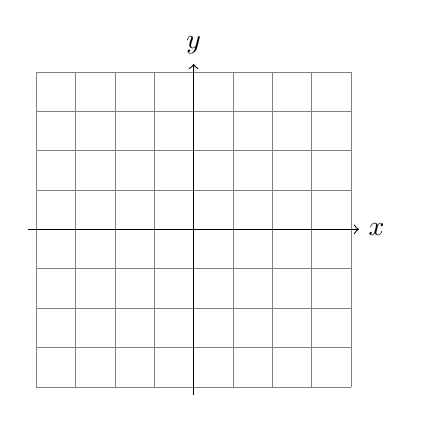
\begin{tikzpicture}[smooth, scale=0.5] %domain=-1.75:1.75, 
    \draw[very thin,color=gray] (-4,-4) grid (4,4);
    \draw[->] (-4.2,0) -- (4.2,0) node[right] {$x$};
    \draw[->] (0,-4.2) -- (0,4.2) node[above] {$y$};
	\clip (-4,-4) rectangle (4,4);
    \draw[color=red] plot[id=x] function{x**3-x} node[right] {};
\end{tikzpicture}
}
\kk{y=x^3-x}{x**3-2*x}{2}
\end{kortit}

%\begin{kortit}{M} %pari, muutama aksioomaa ja laskusääntöä, ei käänteislukua tai osittelulakia, kertolasku luonnollisilla
%
%\k{x-y}{-y+x}
%\k{x-y-x}{-y}
%\k{x+x-x+x}{2x}
%\k{x}{x(2-1)}
%\k{(x+y)-x}{x+(y-x)}
%\k{-x+(x+y)}{y}
%\k{-[(-x)\cdot y]}{yx}
%\k{y\cdot(-x)}{-(xy)}
%\k{(-2)[(-x)\cdot y]}{2xy}
%\k{[(-2)(-1)]\cdot 2}{4}
%\k{-[(-x)\cdot (-y)]}{-(yz)}
%\k{-(-x)\cdot [-(-y)]}{xy}
%\k{(-x)(-y)(-z)}{-xyz}
%\k{(-2x)(-2y)(-2z)}{-8xyz}
%\k{(-2)[x(-y)]}{2xy}
%\k{(-2)[x(-y)]}{[x(-2)](-y)}
%\k{-(2z)\cdot(-(xy)}{2zyx}
%\k{(x+y)-x+(-y)}{0}
%\end{kortit}

%\begin{kortit}{F}
%\k{V(r)=\dfrac{4}{3}\pi r^3}{\mathbb{R}_+ \rightarrow \mathbb{R}_+}
%\k{v(t)=\dfrac{s}{t}}{\mathbb{R}_+ \rightarrow \mathbb{R}}
%\k{v(s)=\dfrac{s}{t}}{\mathbb{R} \rightarrow \mathbb{R}}
%\k{s(t)=vt}{\mathbb{R}_+ \rightarrow \mathbb{R}}
%\k{s(v)=vt}{\mathbb{R} \rightarrow \mathbb{R}}
%\k{F(m)=ma}{\mathbb{R}_+ \rightarrow \mathbb{R}}
%\k{T(l)=2\pi \sqrt{\dfrac{l}{g}}  }{\mathbb{R}_+ \rightarrow \mathbb{R}_+}
%\k{\rho(m)=\dfrac{m}{V} }{\mathbb{R}_+ \rightarrow \mathbb{R}_+}
%\k{\rho(V)=\dfrac{m}{V}}{\mathbb{R}_+ \rightarrow \mathbb{R}_+}
%\k{ N(V)=\rho V g}{\mathbb{R}_+ \rightarrow \mathbb{R}_+}
%\k{ E(v)=\dfrac{1}{2}mv^2}{\mathbb{R} \rightarrow \mathbb{R}_+}
%\k{ P(t)=\dfrac{E}{t}}{\mathbb{R}_+ \rightarrow \mathbb{R}_+}
%\k{F(r)=\gamma \dfrac{m_1m_2}{r^2} }{\mathbb{R}_+ \rightarrow \mathbb{R}_+}
%\k{ \lambda(m)=\left( R_\mathrm{H} \left(\dfrac{1}{m^2}-\dfrac{1}{n^2}\right) \right)^{-1} $\vfill$ R_\mathrm{H}>0 $\vfill$ m,n\in \mathbb{N} }{\mathbb{N} \rightarrow \mathbb{R}_+}
%\k{E(m)=mc^2$ \vfill $\mathrm{c=valonnopeus}}{\mathbb{R}_+ \rightarrow \mathbb{R}_+}
%\k{T_{\frac{1}{2}}(\lambda)=\dfrac{\ln 2}{\lambda} $ \vfill $ \lambda>0}{\mathbb{R}_+ \rightarrow \mathbb{R}_+}
%\k{N(t)=N_0e^{-\lambda t}$ \vfill $\lambda, N_0>0}{\mathbb{R}_+ \rightarrow \mathbb{R}_+}
%\k{f(b)=\left(\dfrac{1}{a}+\dfrac{1}{b}\right)^{-1} $\vfill$ a,b\in \mathbb{R}\setminus \lbrace 0 \rbrace}{\mathbb{R}\setminus \lbrace 0 \rbrace \rightarrow \mathbb{R} \setminus \lbrace 0 \rbrace}
%\end{kortit}

